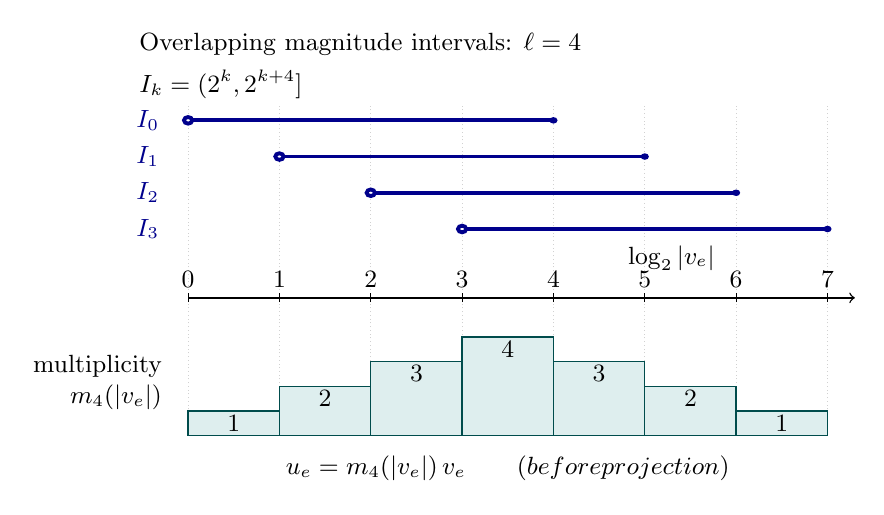
\begin{tikzpicture}[x=1.16cm,y=0.92cm,font=\small,
  every node/.style={inner sep=2pt},
  interval/.style={draw=blue!55!black,line width=1.4pt},
  guide/.style={draw=black!18,densely dotted,line width=0.35pt}]
  \node[anchor=west] at (-0.6,5.4)
    {Overlapping magnitude intervals: $\ell=4$};
  \node[anchor=west] at (-0.6,4.85)
    {$I_k=(2^k,2^{k+4}]$};
  \foreach \j in {0,...,7}{
    \draw[guide] (\j,0) -- (\j,4.55);
  }
  \foreach \k in {0,...,3}{
    \pgfmathsetmacro{\rightend}{\k+4}
    \pgfmathsetmacro{\rowheight}{4.35-0.5*\k}
    \node[anchor=east,text=blue!55!black] at (-0.25,\rowheight)
      {$I_{\k}$};
    \draw[interval] (\k,\rowheight) -- (\rightend,\rowheight);
    \draw[interval,fill=white] (\k,\rowheight) circle[radius=0.045];
    \fill[blue!55!black] (\rightend,\rowheight) circle[radius=0.045];
  }
  \draw[->,line width=0.5pt] (0,1.9) -- (7.3,1.9);
  \foreach \j in {0,...,7}{
    \draw (\j,1.84) -- (\j,1.96);
    \node[above] at (\j,1.96) {$\j$};
  }
  \node[anchor=west] at (4.75,2.45) {$\log_2|v_e|$};
  \foreach \j/\mult in {0/1,1/2,2/3,3/4,4/3,5/2,6/1}{
    \pgfmathsetmacro{\rightbin}{\j+1}
    \pgfmathsetmacro{\barheight}{0.34*\mult}
    \filldraw[fill=teal!13,draw=teal!60!black,line width=0.5pt]
      (\j,0) rectangle (\rightbin,\barheight);
    \node at ({\j+0.5},{\barheight-0.17}) {$\mult$};
  }
  \node[anchor=east,align=right] at (-0.22,0.73)
    {multiplicity\\$m_4(|v_e|)$};
  \node[anchor=north] at (3.5,-0.2)
    {$u_e=m_4(|v_e|)\,v_e\qquad\text{(before projection)}$};
\end{tikzpicture}
